
\begin{frame}\frametitle{Results}
  \setbeamercovered{invisible}

\begin{figure}
\centering
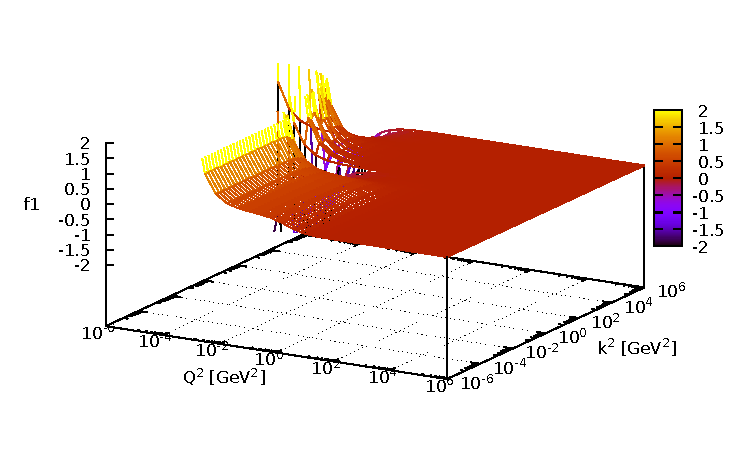
\includegraphics[width=0.7\linewidth]{f1.svg}
\caption{}
\label{}
\end{figure}

\end{frame}

\begin{frame}\frametitle{Results}
  \setbeamercovered{invisible}

\begin{figure}
\centering
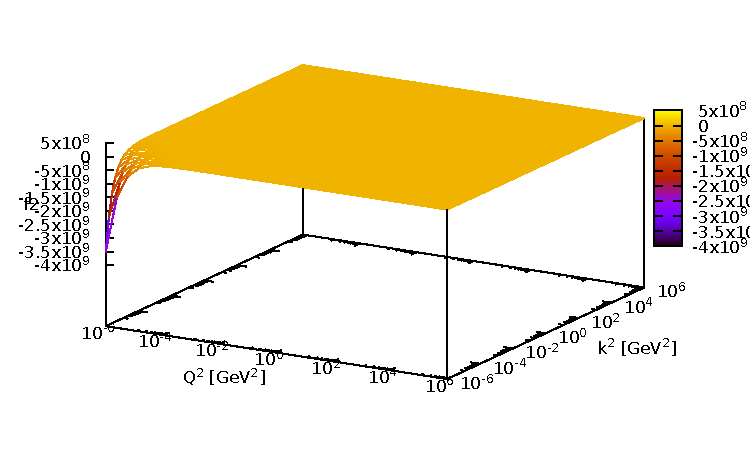
\includegraphics[width=0.7\linewidth]{f2.svg}
\caption{}
\label{}
\end{figure}

\end{frame}

\begin{frame}\frametitle{Results}
  \setbeamercovered{invisible}

\begin{figure}
\centering
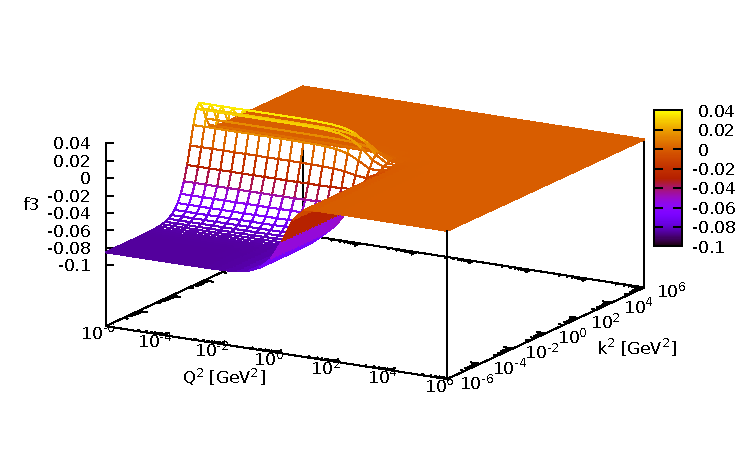
\includegraphics[width=0.7\linewidth]{f3.svg}
\caption{}
\label{}
\end{figure}

\end{frame}

\begin{frame}\frametitle{Results}
  \setbeamercovered{invisible}

\begin{figure}
\centering
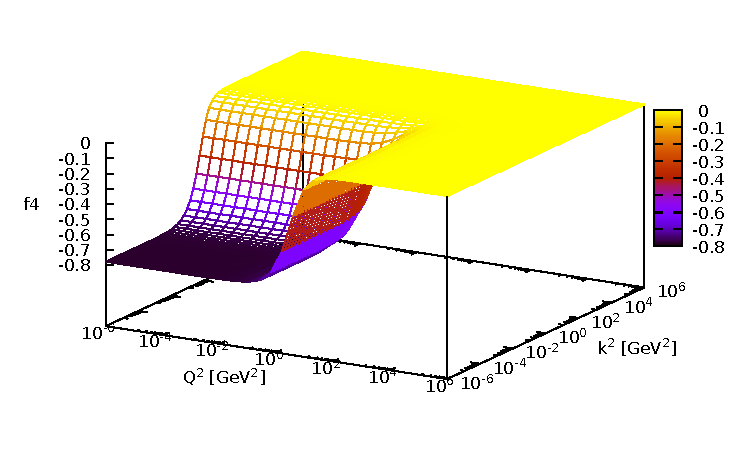
\includegraphics[width=0.7\linewidth]{f4.svg}
\caption{}
\label{}
\end{figure}

\end{frame}

\begin{frame}\frametitle{Results}
  \setbeamercovered{invisible}

\begin{figure}
\centering
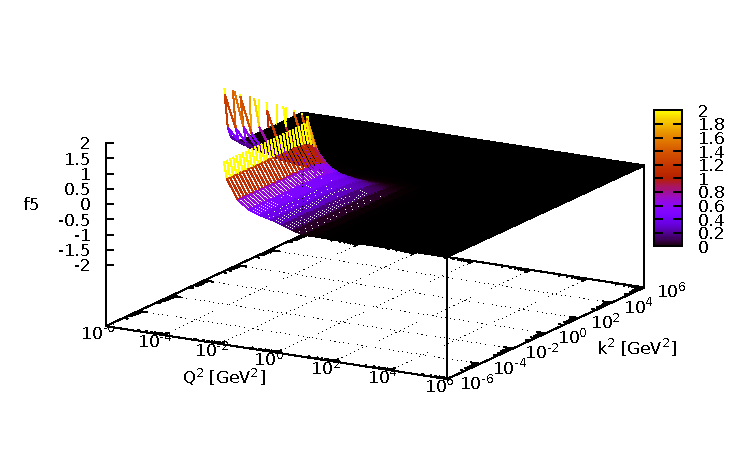
\includegraphics[width=0.7\linewidth]{f5.svg}
\caption{}
\label{}
\end{figure}

\end{frame}

\begin{frame}\frametitle{Results}
  \setbeamercovered{invisible}

\begin{figure}
\centering
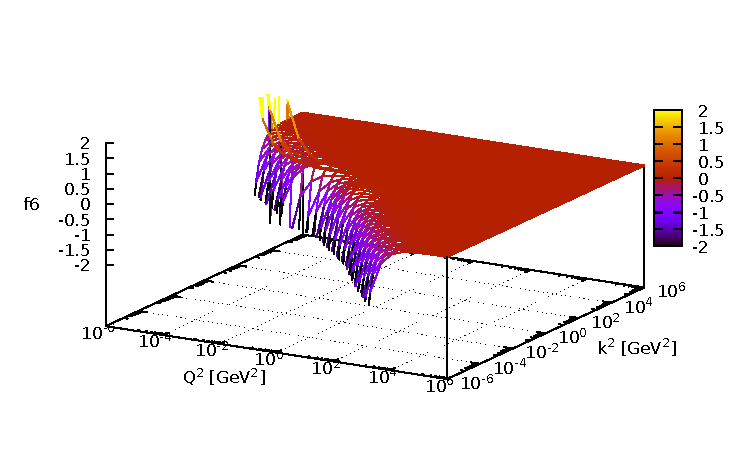
\includegraphics[width=0.7\linewidth]{f6.svg}
\caption{}
\label{}
\end{figure}

\end{frame}


\begin{frame}\frametitle{Results}
\begin{figure}
\centering
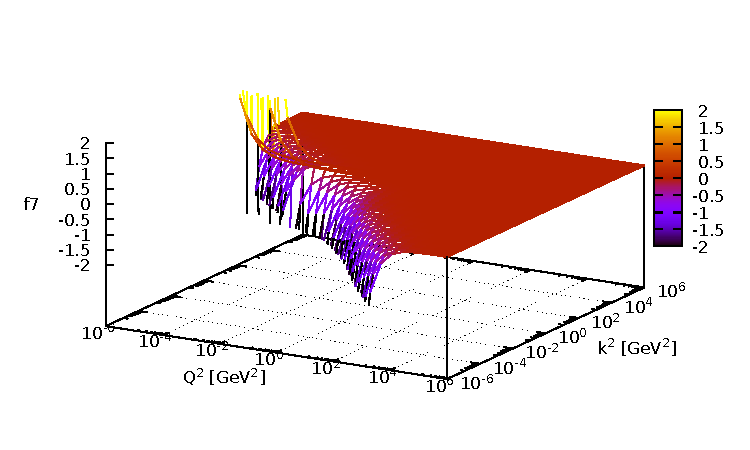
\includegraphics[width=0.7\linewidth]{f7.svg}
\caption{}
\label{}
\end{figure}

\end{frame}

\begin{frame}\frametitle{Results}
\begin{figure}
\centering
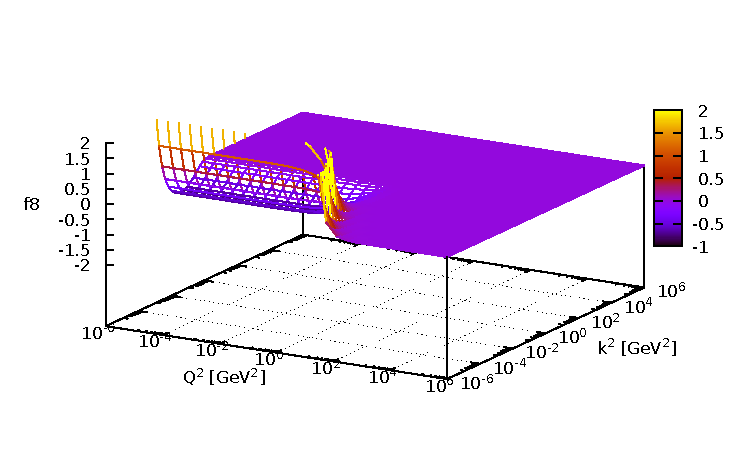
\includegraphics[width=0.7\linewidth]{f8.svg}
\caption{}
\label{}
\end{figure}
\end{frame}

\begin{frame}\frametitle{Results}
\begin{figure}
\centering
\includegraphics[width=0.7\linewidth]{f9.svg}
\caption{}
\label{}
\end{figure}
\end{frame}

\begin{frame}\frametitle{Results}
\begin{figure}
\centering
\includegraphics[width=0.7\linewidth]{f10.svg}
\caption{}
\label{}
\end{figure}
\end{frame}

\begin{frame}\frametitle{Results}
\begin{figure}
\centering
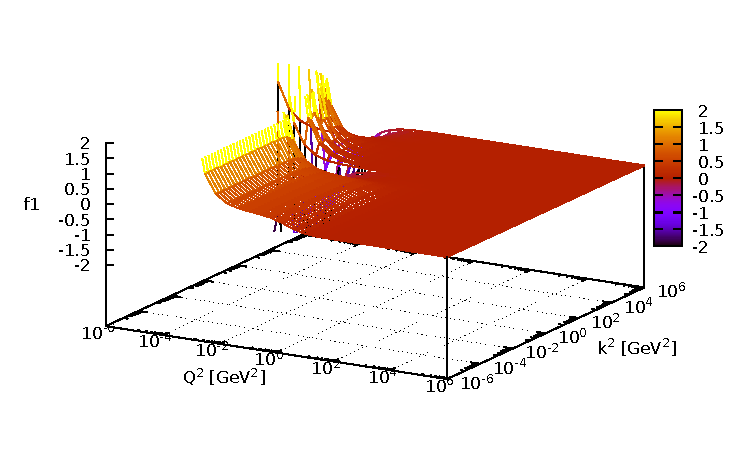
\includegraphics[width=0.7\linewidth]{f1.svg}
\caption{}
\label{}
\end{figure}
\end{frame}

\begin{frame}\frametitle{Results}
\begin{figure}
\centering
\includegraphics[width=0.7\linewidth]{WT1.svg}
\caption{}
\label{}
\end{figure}
\end{frame}

\begin{frame}\frametitle{Results}
  \setbeamercovered{invisible}

\begin{figure}
\centering
\includegraphics[width=0.7\linewidth]{WT2.svg}
\caption{}
\label{}
\end{figure}

\end{frame}

\begin{frame}\frametitle{Results}
  \setbeamercovered{invisible}

\begin{figure}
\centering
\includegraphics[width=0.7\linewidth]{WT3.svg}
\caption{}
\label{}
\end{figure}

\end{frame}

\begin{frame}\frametitle{Results}
  \setbeamercovered{invisible}

\begin{figure}
\centering
\includegraphics[width=0.7\linewidth]{WT4.svg}
\caption{}
\label{}
\end{figure}

\end{frame}

\endinput